\documentclass{article}

\usepackage{graphicx}
\usepackage{float}
\graphicspath{ {./images/} }

\author{Erik-Cristian seulean}
\title{Nonparametric bayesian inference - a guide to clustering algorithms}
\date{\today}

\begin{document}
\maketitle
\section{Motivation}

In the last years, in every corner of the internet there are enormous quantities of data created. 
Regardless of the nature of this data, as quantities increase over time, we're challenged to find
ways to group data into well defined categories. The categorisation of data allows us to explore 
datasets in a more organised way and reduces the time required to find particular datapoints. 
Today, there are over 6 million articles on Wikipedia. Regardless of the vastity of this article
collection, everything is grouped in ways that allows us to explore different interests in
organised ways. The library, here in St. Andrews contains over 1 million books, yet finding a book
today on a topic such as Bayesian inference is a matter of minutes. As the University increases the
diversity of degrees that students can take, the number of book categories increase over time and 
this leads to the following question \textit{How do we generate a mathematical model that is capable
to group future books given the collection of books currently available ?}

\section{Nonparametric Bayes a brief description}
There are two separate classes of Bayesian inference. One class contains inference on
parameters of distributions, where the prior and posterior distributions are functions of parameters of
interest with fixed dimension. In this case we can consider the following: 

\begin{itemize}
    \item $\theta = (\theta_{1}, \theta_{2}, ..., \theta_{n})$ - the parameter that we are interested in 
    \item $P(\theta)$ - prior probability
    \item $\pi(\theta|X)$ - posterior probability
\end{itemize}

In the above example, the parameter has a fixed determined dimension. We know what probability distributions
work for the number of parameters we have. For a single unknown parameter we can for example use a Uniform, 
Poission or Exponential distribution. For two parameters we could use a Normal or Beta distribution (among others)
depending what sort of data we are modelling. 
In this situation we can use Bayes formula to define the posterior distribution based on the prior and likelihood:

$$\pi(\theta|x_{1}, x_{2}, ..., x_{n}) \propto \prod_{i}^{n}f(x_{i}|\theta)p(\theta)$$


But what happens when you don't know beforehand how many parameters you need ? How many parameters will describe
your data well ? Are your observations dependent on one parameter or 3 parameters ? Nonparametric Bayesian analysis
is focused on problems where the number of parameters are not known beforehand. In other words, we can assume that
there can be any number of parameters, we will examine the data and draw some conclusions on how many parameters of 
interest describe the data well. 
In more righourous mathematical terms, so far we can define the following:

\begin{itemize}
    \item $X_{1}, X_{2}, X_{3}, ... X_{n}$ are i.i.d observations from an \textit{unknown} distribution F
    \item F is not from a finite space, we cannot index it with a finite number of parameters
\end{itemize}

Similar to the parametric case, we would like to apply Bayesian methods. This means that we need to 
specify a prior distribution, but because we don't know the number of parameters that we are dealing with,
we cannot specify priors on parameters, we need to specify a prior on the distribution itself. What in 
the parametric case was $P(\theta)$ becomes now $P(F)$ where F is a distribution! 
To put it in the context of the example from the beginning of the essay, if we start making an analysis on
the topics of the books in the library, the more books we examine the more topics we can encounter. That doesn't
mean that every book is a new topic, but the number of topics grows as we examine more books. This is equivalent
to the number of parameters in a nonparametric Bayesian model where the number of parameters is unknown but growing
with the data. 

\section{The clustering problem}
Assuming we have observations $X_{1}, X_{2}, ..., X_{n}$ we want to assign every datapoint to a single cluster.

\begin{figure} [H]
    \begin{center}
        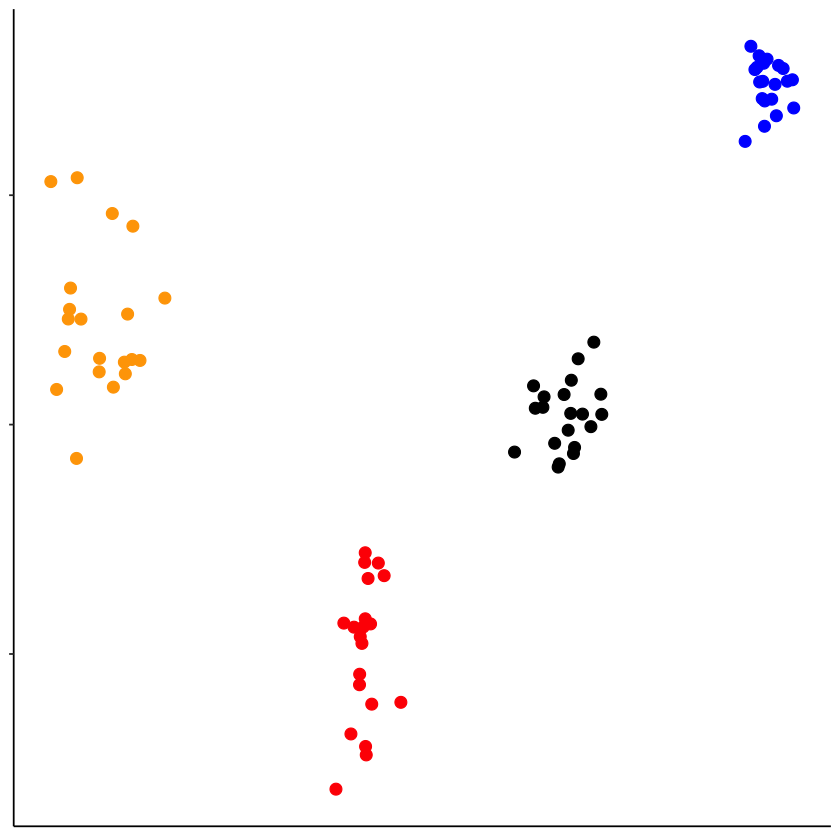
\includegraphics[scale=0.3, width=5cm]{clusters.png}
        \caption{Clustered datapoints}
        \label{fig:boat1}
    \end{center}
\end{figure}

In a general Gaussian mixture model, with the number of clusters $K$ set to 2, we could potentially have the following setup: 

$$\mu_{k} \sim \mathcal{N}(\mu_{0}, \sigma_{0})$$ 
$$\rho_{1} \sim Beta(a, b)$$
$$\rho_{2} = 1 - \rho{1}$$ 
$$Z_{n} \sim Categorical(\rho_{1}, \rho_{2})$$
Here we're choosing $\rho_{1}$ coming from a Beta distribution as it is mathematically convenient, but in practice, it would require further analysis to figure out if this is a valid assumption. Depending on the parameters of this Beta distribution, it would put more or less mass on $\rho_{1}$ compared to $\rho_{2}$.

In case we want to generalise the model above to have K clusters, we can replace the Beta distribution above with a Dirichlet distribution. In this case, instead of drawing only one observation for $\rho_{1}$, we could draw K observation for $\rho_{1}, \rho_{2}, \rho_{3}, ..., \rho_{K}$.

$$\mu_{k} \sim \mathcal{N}(\mu_{0}, \sigma_{0})$$ 
$$\rho_{1:K} \sim Dirichlet(a_{1}, a_{2}, ..., a_{K})$$
$$Z_{n} \sim Categorical(\rho_{1}, \rho_{2}, ... ,\rho_{K})$$

The Dirichlet distribution used above is the natural generalisation of Beta distribution to a multiparameter case:

$$ Dir(\rho_{1}, \rho_{2}, ..., \rho_{n}| a_{1}, a_{2}, ..., a_{n}) = \frac{\Gamma(\sum_{i=1}^{K}a_{i})}{\prod_{i=1}^{K}\Gamma(a_{i})}\prod_{i}^{K}\rho_{i}^{a_{i} - 1}$$ where
$\sum_{i}^{K} \rho_{i} = 1, a_{k} > 0$ and $\rho_{k} \in (0, 1)$.

The \textit{rdirichlet} function provided with the library can generate samples from a Dirichlet distribution.

So far the examples above, all work on the case where the number of clusters is fixed and known. We are capable of drawing observations from the Dirichlet distribution, because we know how many parameters we are working with. In the figure below, the first delimitation corresponds to the first cluster, second to the second cluster and so on, up to 100 clusters.

\begin{figure} [H]
    \begin{center}
        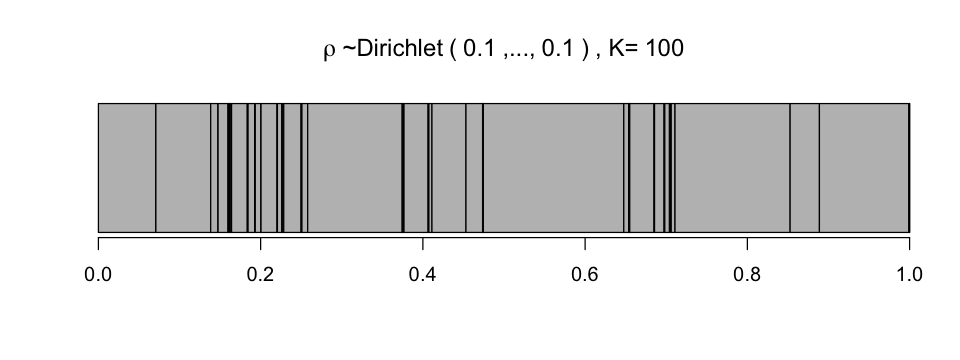
\includegraphics[scale=1, width=5cm]{stacked_dirichlet.png}
        \caption{Clusters generated from a Dirichlet distribution.}
        \label{fig:stacked_dirichlet}
    \end{center}
\end{figure}

At this point, we only considered the available clusters, but we have not sampled our datapoints $X_{1}, X_{2}, ..., X_{n}$ into the corresponding clusters. To put a particular datapoint into a certain cluster, we can draw an observation from a Uniform distribution and check which cluster it belongs to. We can repeat the same until all n datapoints are assigned to a cluster. The cluster generation function in the library allows to visually get an intuition of how this happens sequentially. 

\begin{figure} [H]
    \begin{center}
        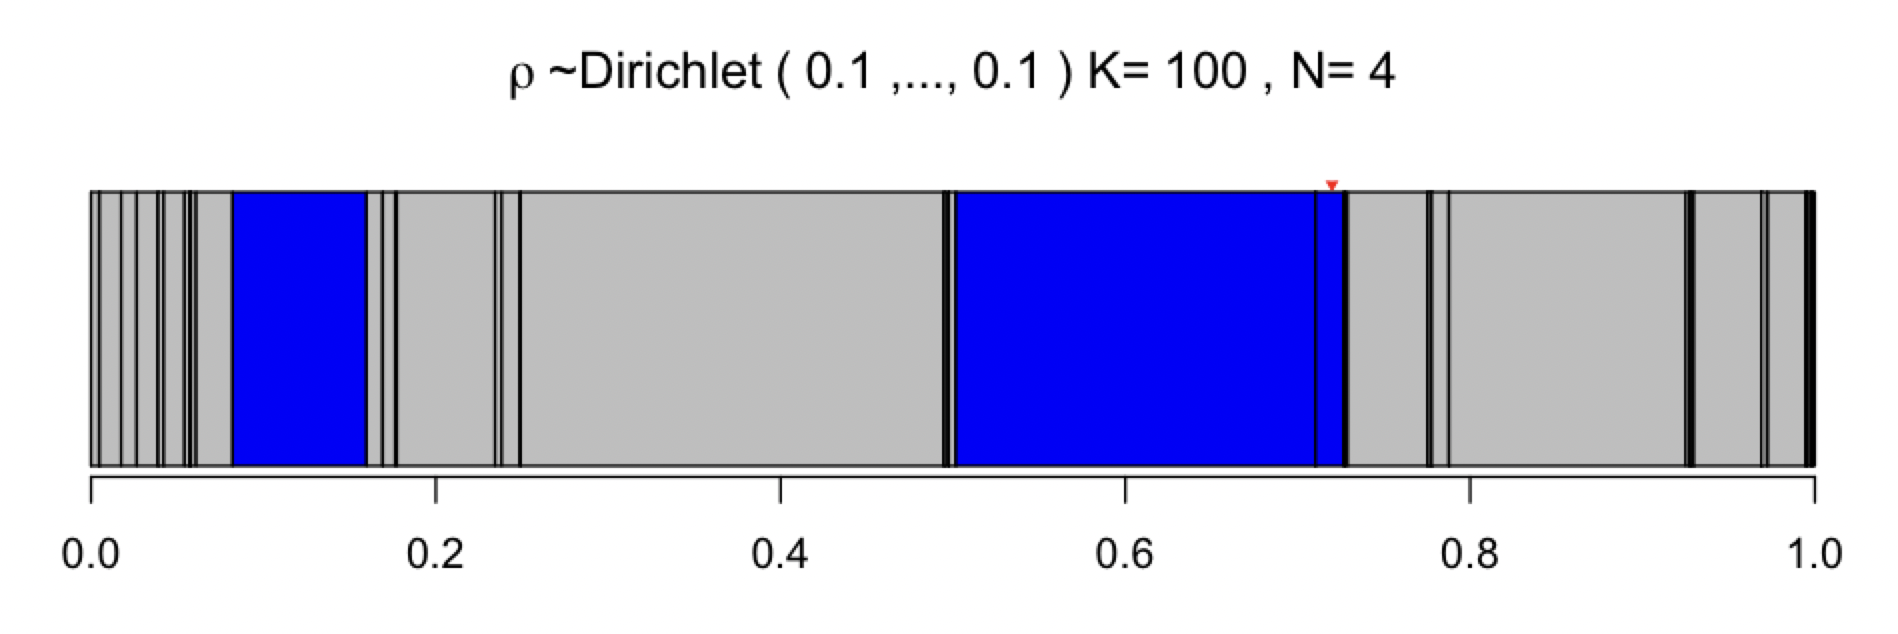
\includegraphics[scale=1, width=5cm]{clustered_points.png}
        \caption{Clustered points}
        \label{fig:clustered_points}
    \end{center}
\end{figure}

While this model looks appealing, there is always going to be an upper bound on K, that defines the number of clusters. In this scenario, there is no reliable way to choose K that would be sufficient in any general case. Even if we can come up with a value of K large enough, there are computational concerns when it comes to storing a large amount of information in memory that is associated with K.

\section{Setting K=$\infty$}
A solution to the above limitation is to set K to be arbitrary large that would not limit us from having a very large number of clusters. In this case we need a different procedure to generate $\rho_{1}, \rho_{2}, ..., \rho_{K}$ from a Dirichlet distribution. What we want to do is take the interval $(0, 1)$ and break it into an infinite number of subintervals that sum up to 1. In other words, we first break a proportion of the interval $(0, 1)$ and denote that being $\rho_{1}$. Out of the remaining part $(\rho_{1}, 1)$ we break another proportion and denote that to be $\rho_{2}$. We can repeat this as many times as we want and we can generate an infinite number of proportions, that sum up to 1, the length of the initial interval. This algorithm is called the \textit{"stick-breaking process"} and can be sumarised as follows: 

\begin{itemize}
    \item Generate $P_{1} \sim Beta(a_{1}, b_{1})$. Set $\rho_{1}$ to this value.  
    \item Generate $P_{2} \sim Beta(a_{2}, b_{2})$. Set $\rho_{2} = (1 - P_{1})P_{2}$
    \item Generate $P_{3} \sim Beta(a_{3}, b_{3})$. Set $\rho_{3} = (1 - P_{1})(1-P_{2})P_{3}$
    \item Set $\rho_{K} = 1 - (\rho_{1} + \rho_{2} + ... + \rho_{K-1})$
\end{itemize}

The choice of parameters $a$ and $b$ for the Beta distribution are researched by Ishwaran and James, 2001, and we will simply use $1$ and $\alpha$ with $\alpha$ given for all $\alpha_{k}$ and $\beta_{k}$. 
When $a_{k}=1$ and $b_{k}=\alpha$, $\alpha > 0$ the process is called \textit{Dirichlet process stick-breaking}. The distribution over all $\rho = (\rho_{1}, \rho_{2}, ...)$ is called Griffin-Engen-McCloskey (GEM). 

$$ (\rho_{1}, \rho_{2}, ...) \sim GEM(\alpha)$$

\end{document}\models